\documentclass[titlepage,12pt]{article}
\usepackage[unicode]{hyperref} 
\usepackage{amsmath,epsfig,pifont,calc,pifont}	
\usepackage{float} 
\usepackage{rom}
\usepackage[romanian]{babel}
\usepackage{amsmath}
\usepackage{multicol}
\usepackage{array}
\usepackage{listings}
\usepackage{color}
\usepackage{graphicx}
\graphicspath{ {images/} }


\definecolor{codegray}{rgb}{0.5,0.5,0.5}
\definecolor{codepurple}{rgb}{0.58,0,0.82}
\definecolor{backcolour}{rgb}{1,1,1}

\setlength{\parindent}{3ex} 
\setlength{\voffset}{-2cm}
\setlength{\textheight}{23cm}  
\setlength{\textwidth}{16cm}
\setlength{\topmargin}{0cm}
\setlength{\headsep}{1cm}
\setlength{\oddsidemargin}{0.5cm}
\setlength{\evensidemargin}{-0.3cm}
\raggedbottom
\renewcommand{\contentsname}{Cuprins}
\renewcommand{\figurename}{Figura}
\renewcommand\refname{Bibliografie 'si Webografie}
\renewcommand\labelenumi{(\theenumi)}

\numberwithin{figure}{section}

\usepackage[utf8]{inputenc}
 
\setlength{\arrayrulewidth}{1mm}
\setlength{\tabcolsep}{18pt}
\renewcommand{\arraystretch}{1.5}

\lstdefinestyle{stilmatlab}{
  backgroundcolor=\color{backcolour},
  commentstyle=\color{blue},
  keywordstyle=\color{magenta},
  numberstyle=\tiny\color{codegray},
  stringstyle=\color{codepurple},
  basicstyle=\footnotesize,
  breakatwhitespace=false,         
  breaklines=true,                 
  captionpos=b,                    
  keepspaces=true,                 
  numbers=left,                    
  numbersep=5pt,                  
  showspaces=false,                
  showstringspaces=false,
  showtabs=false,                  
  tabsize=2
}	

\lstset{style=stilmatlab}

\hypersetup{
    colorlinks=false,
    pdfborder={0 0 0},
}

\pagestyle{plain}
 
\begin{document}
\title{Tem'a\\
{\small - la disciplina "Analiza Algoritmilor" - \\
- Structuri de date - \\- AVL 'si Binary Heap - \\ - Cozi de prioritate -}}
\author{{ Iona'scu Andrei} \\ Anul II \\
 325CD \\ Facultatea de Automatic'a 'si Calculatoare \\ Universitatea Politehnic'a Bucure'sti}
\maketitle

\newpage
\tableofcontents

\newpage
\section{Introducere}
\subsection{Prezentarea algoritmilor} 
\par Pentru aceast'a tem'a am ales s'a studiez structurile de date, mai exact, cozi de prioritate.
Voi aduce spre implementare la categoria arbori binari echilibra'ti,algoritmul AVL, iar la categoria heap, algoritmul Binary heap. \par
\subsubsection{AVL tree}
	AVL tree-ul este un arbore binar echilibrat, care urm'are'ste acelea'si propriet'a'ti ca 'si un arbore binar de c'autare: fiecare nod din subarborele st\^ang prezint'a o valoare mai mic'a dec\^at nodul r'ad'acin'a, iar fiecare r'ad'acin'a din subarborele drept prezint'a o valoare mai mare dec\^at nodul r'ad'acin'a. 
	\par Avantajul AVL-ului vine prin abilitatea sa de a se echilibra, av\^and 'in fiecare moment, un arbore echilibrat, cu ajutorul factorilor de echilibrare ('intre -1 'si 1). 
	\par Datorit'a acestei abilit'a'ti, AVL-ul prezint'a o complexitate de \textbf{$\mathcal{O}(log N)$} at\^at 'in momentul inser'arii, c\^at 'si la 'stergerea 'si c'autarea unui num'ar. 
\subsubsection{Binary Heap}
Binary Heap-ul este o structur'a de tip heap ce ia forma unui binary tree. Pe l'ang'a atributele unui binary tree, aceast'a structur'a prezint'a 'inc'a dou'a propriet'a'ti: aceasta este un arbore binar complet (toate nivele sunt complete, iar ultimul este completat de la st'anga la dreapta) 'si cheia stocat'a 'in fiecare nod este mai mare sau egal'a (mai mic'a sau egal'a) cu cheia din nodul copil, 'in func'tie de implementare. 
	\par Datorit'a acestor propriet'a'ti, Binary Heap-ul prezint'a o complexitate la inserare de \textbf{$\mathcal{O}(log N)$} pe cazul cel mai defavorabil, 'si $\mathcal{O}(1)$ pe cazul mediu, la 'stergerea unui element $\mathcal{O}(log N)$ 'in ambele cazuri 'si la c'autare $\mathcal{O}(N)$.

\subsection{Compararea algoritmilor} 
\par Implementarea acestor dou'a structuri prezint'a at'at avantaje, c'at 'si dezavantaje pe anumite opera'tii, neput'and s'a spunem c'a unul dintre ace'sti algoritmi este cu mult mai bun, pe toate planurile, fa't'a de cel'alalt.
\par Astfel, algoritmul AVL este bun pe opera'tii de c'autare, datorit'a abilit'a'tii acestuia de a se echilibra. Algoritmul Binary Heap este implementat adesea pe baza unui array. Stiind c'a num'arul maxim(minim) din arbore se va afla in nodul root, 'in func'tie de tipul de Binary heap (minHeap sau maxHeap), acesta poate fi returnat imediat, cu o complexitate de $\mathcal{O}(1)$, 'stiind c'a acesta se afl'a pe pozi'tia 0 'in array. De asemenea, dac'a 'in aceast'a structur'a sunt inserate elemente deja sortate (aproape sortate), complexitatea inser'ari elementelor tinde spre $\mathcal{O}(1)$, pe c\^and la AVL este nevoie ca dup'a fiecare inserare s'a se echilibreze arborele, indiferent de oridinea inser'arii, dac'a este nevoie.

\subsection{Situa'tii practice} 
Pentru a pune 'in eviden't'a atuurile fiec'arui algoritm, putem considera urm'atoarele exemple practice generice:
	\par - AVL va fi implementat atunci c'and 'stim c'a vom avea nevoie de interog'ari multiple asupra tuturor nodurilor, c'autarea acestora fiind de complexitate $\mathcal{O}(log N)$, deoarece este echilibrat.
	\par - Binary Heap va fi implementat atunci c'and 'stim c'a vom avea nevoie de interog'ari asupra minimului sau maximului (minHeap sau maxHeap), deoarece ace'stia pot fi apela'ti 'in timp $\mathcal{O}(1)$, deoarece ace'stia se afl'a pe pozi'tia 0 'in structur'a.
	\\ \par Pentru a v'a oferi un exemplu complex, pot folosi aceste structuri 'in cadrul unui campionat de Karate, unde, doresc s'a men'tin ierarhi cu concuren'ti 'si s'a realizez statistici.
	\par Cu ajutorul AVL-ului voi putea men'tine ierarhiile cu sportivi sorta'ti dup'a un anumit criteriu, put\^and s'a accesez rapid datele acestor sportivi.
	\par Cu ajutorul Binary heap-ului voi putea realiza multiple statistici pe parcursul competi'tiei, 'in care voi urm'ari cei mai buni/cei mai slabi concuren'ti, 'in func'tie de lupte c'a'stigate, puncte (tot ce 'tine de interogarea minimului/maximului).
	
\section{Complexitate}	
\subsection{AVL tree}
\subsubsection{Temporal'a}
\textbf{Temporal}, AVL prezint'a pe insert, find, c\^at 'si delete, o complexitate  $\mathcal{O}(log N)$. Stiind c'a la fiecare inserare, arborele se va verifica dac'a mai este echilibrat 'si va realiza opera'tii de echilibrare, acestea nu prezint'a un impact asupra timpului de execu'tie, fiind realizate pu'tine mut'ari 'in structur'a. Complexitatea acestuia este dat'a de nevoie de inserare a celor N elemente 'intr-un arbore binar de c'autare, reprezentat'a de 'in'al'timea acestui arbore. 'In'al'timea unui arbore binar echilibrat este logN, rezult\^and o complexitate total'a de  $\mathcal{O}(log N)$. 
\par Aceea'si logic'a este prezent'a 'si 'in cadrul c'aut'arii 'si al 'stergerii. Pentru a c'auta un element ('si a-l 'sterge) 'in arbore, programul va trebui s'a parcurg'a aproape 'intreg arborele, sau chiar 'in totalitate, fiind de 'in'al'time logN, iar c\^and s-a ajuns la nodul dorit, 'in cazul 'in care dorim eliminarea acestuia, programul va realiza mici echilibr'ari nesemnificative 'in compara'tie cu logN.
\subsubsection{Spa'tial'a}
\par
\textbf{Spa'tial}, AVL prezint'a o complexitate $\mathcal{O}(1)$, deoarece acesta va aloca memorie o singur'a dat'a pentru fiecare nod din interiorul arborelui, f'ar'a a avea nevoie de spa'tiu suplimentar.

\subsection{Binary Heap}
\subsubsection{Temporal'a}
Pe partea de insert, Binary Heap prezint'a pe worst case, o complexitate $\mathcal{O}(logN)$, deoarece, la inserarea unui nou element 'in arbore, va trebui pus pe pozi'tia potrivit'a, prin interschimb'ari ale valorilor, prin array. Dac'a introducem un element, acesta va fi plasat prin algoritm, la finalul array-ului, si va trebui s'a sa fie urcat 'in arbore p\^an'a la root, arborele av\^and 'worst case in'al'timea logN, de aici venind 'si complexitatea. Pe cazul mediu, inserarea poate fi chiar $\mathcal{O}(1)$, acesta fiind pozi'tionat chiar unde trebuie, sau 'in vecin'atatea potrivit'a.
\par Algoritmul de 'stergere prezint'a o complexitate de $\mathcal{O}(logN)$, deoarece, dup'a 'stergerea unui element din arbore, acesta va fi 'inlocuit cu ultimul element din array 'si pornind de la acea pozi'tie, trebuie s'a se readuc'a arborele la normal, pentru a-'si p'astra proriet'at'ile. Astfel, elementul de la finalul array-ului, care se afla acum pe pozi'tia elementului eliminat, va trebui s'a parcurg'a arborele p'ana va fi plasat la pozi'tia potrivit'a, arborele av\^and 'inal'timea logN.
\par Algoritmul de c'atuare este de complexitate $\mathcal{O}(N)$, deoarece acesta trebuie trebuie parcurs 'intreg array-ul pentru a g'asi elementul dorit. Acest lucru se datoreaz'a faptului c'a elementele vor fi ad'augate 'in arbore, de la st'anga la dreapta, singura restrictie fiind ca elementul inserat s'a fie mai mic sau egal cu elementul p'arinte. C'autarea elementului maxim (minim) dintr-un MaxHeap (MinHeap) are o complexitate de $\mathcal{O}(1)$, deoarece acesta se va afla pe pozi'tia 0 'in array, prezent'and avantajul acestei structuri.
\subsubsection{Spa'tial'a}
\par \textbf{Spa'tial}, Binary Heap prezint'a complexitatea $\mathcal{O}(1)$, deoarece la ini'tializarea acesteia, se va aloca memorie pentru un array cu N elemente, care va con'tine datele pentru fiecare nod din structur'a, f'ar'a a fi nevoie de memorie auxiliar'a.

\section{Implementare}
\par Codul pentru AVL este implementat 'in java 'si a fost luat de pe site-ul urm'ator\cite{AVL}.
\par Codul pentru Binary Heap este impementat 'in java 'si a fost luat de pe site-ul urm'ator\cite{BIN}.
\par Implement'arile 'si clasele de testare se pot g'asi 'in interiorul arhivei. Implenet'arile algoritmilor se g'asesc la finalul documentului 'in anexa de implementare, deoarece acestea ocup'a o dimensiune foarte mare.

\section{M'asurarea performan'tei}
\par Toate testele au fost realizate pe un set de date pe cazul worst case (datele au fost generate cu ajutorul site-ului Random.org\cite{ran} 'si sunt ordonate descresc'ator). Datele introduse sunt de urm'atoarele dimensiuni: 100, 500, 1000, 2500, 5000, 10000.
\subsection{Performan't'a Insert}
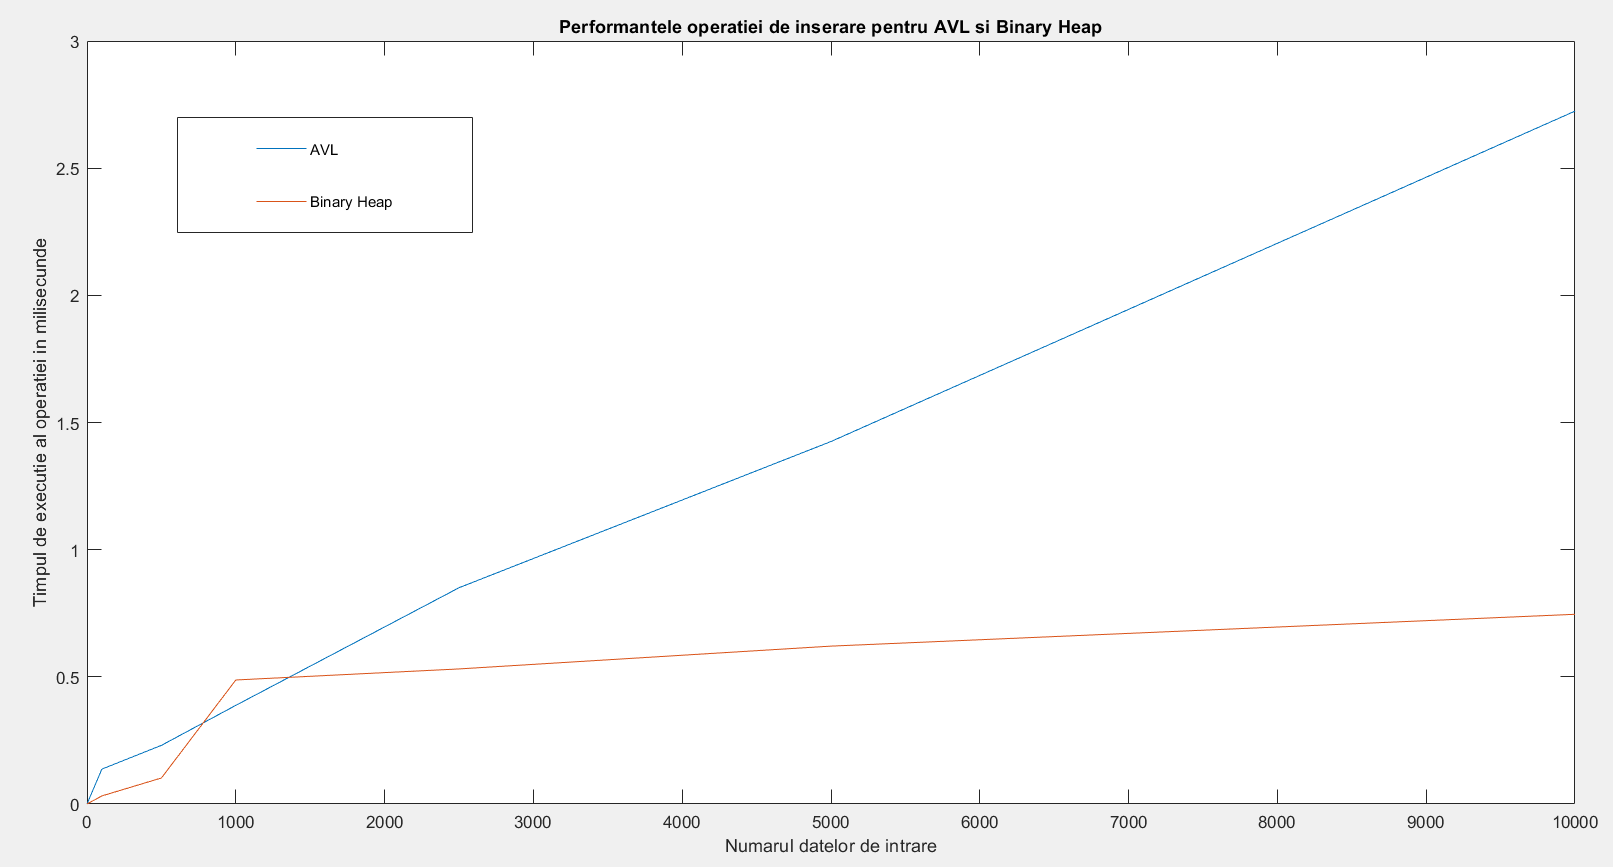
\includegraphics[scale=0.5]{Insert}
\\ \par 'In urma test'arii performan'tei pentru opera'tia de inserare, am ob'tinut graficul de mai sus, 'in care durata de execu'tie a progrmului este 'in milisecunde. 
\par Cu ajutorul acestui grafic putem observa c'a timpul de execu'tie al structurii AVL este cu mult mai 'inceat'a fa't'a de Binary Heap. 
\par Fiecare element nou introdus 'intr-un Binary Heap va fi stocat 'intr-un array, fiind pus la coada array-ului, ca mai apoi s'a se parcurg'a prin p'arin'ti pentru a i se oferi pozi'tia corect'a 'in arbore. Din acest motiv, Binary Heap este mai rapid dec\^at opera'tia de insert din AVL, care, va parcurge de la root fiecare nod, 'in c'autarea locului potrivit, ca mai apoi s'a asigure echilibrarea arborelui, prin rota'tiile necesare.
\par Pute'ti observa 'in imaginea urm'atoare, 'in ce const'a inserarea unui element nou 'in AVL, ce realizeaz'a 'si o dezechilibrare a acestuia, fiind nevoie s'a se re-echilibreze.
\\
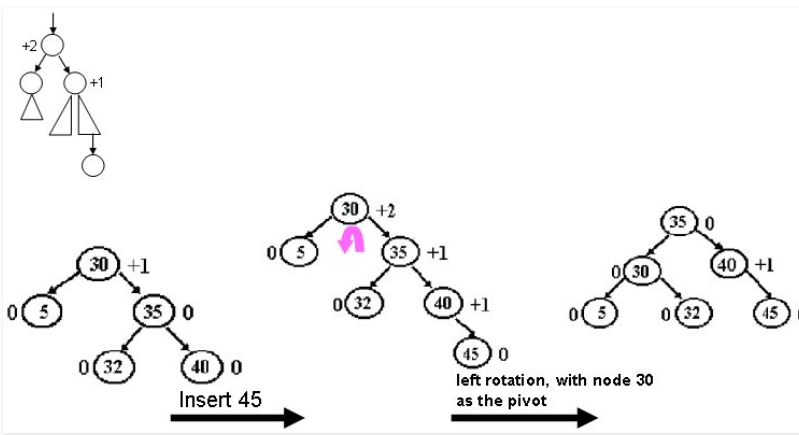
\includegraphics[scale=0.7]{insertex}

\subsection{Performan't'a Find Minimum}
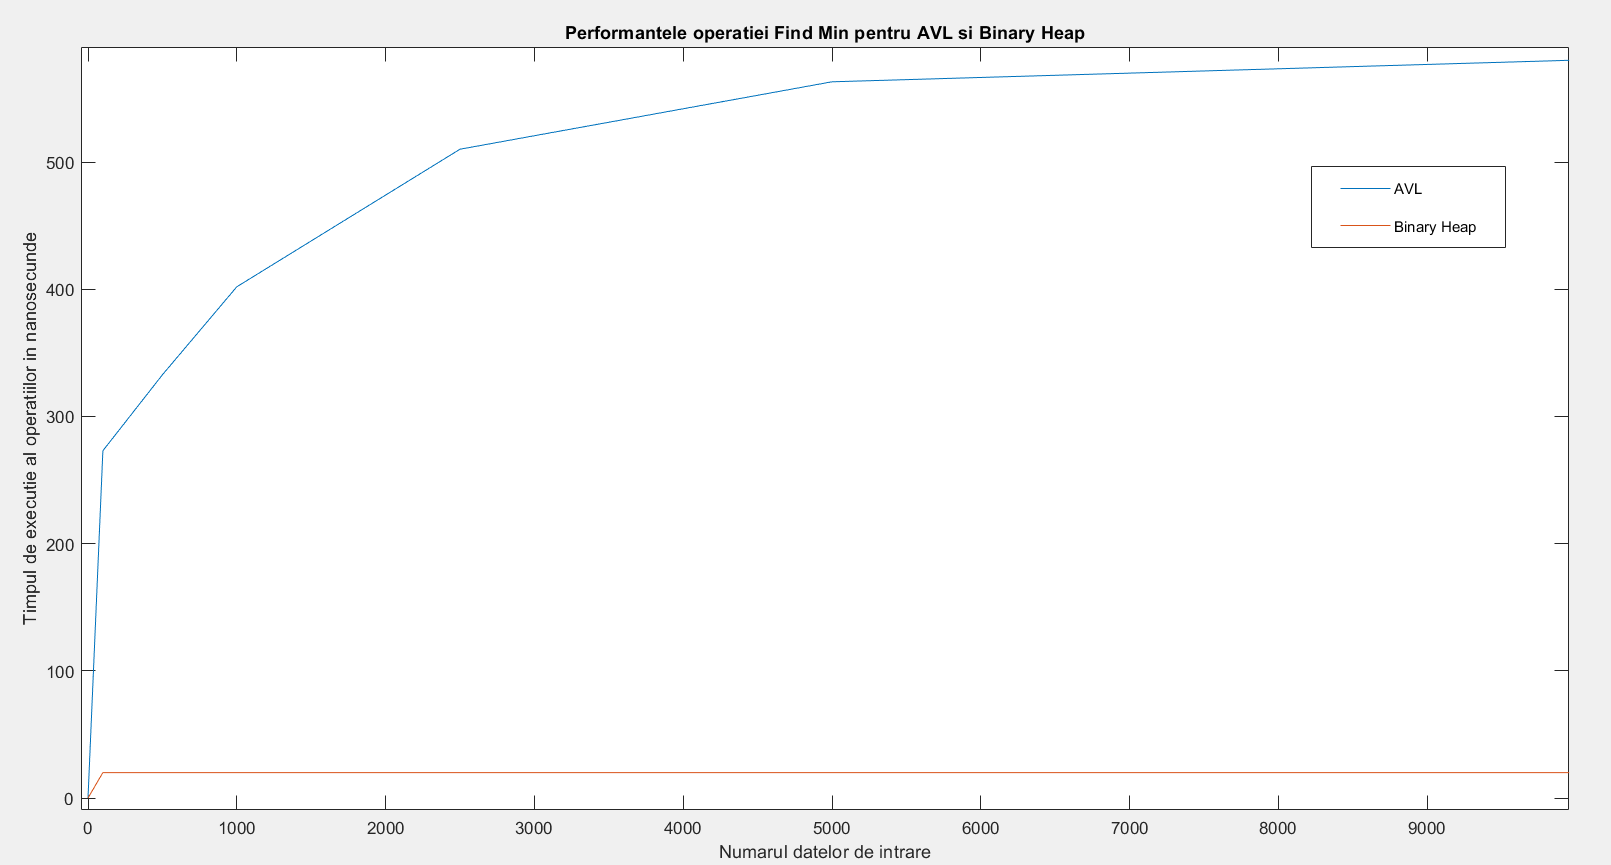
\includegraphics[scale=0.5]{FMin}
\\ \par 'In urma test'arii performan'tei pentru opera'tia de c'autare a elementului minim, am ob'tinut graficul de mai sus, 'in care durata de execu'tie a progrmului este 'in nanosecunde. 
\par Pe acest grafic se poate observa atuu-ul structurii Binary Heap (MinHeap), care ofer'a termenul minim instant, deoarece acesta se afl'a 'in nodul root, pe pozi'tia 0 din array-ul arborelui. Pentru a elimina elementul minim dintr-un AVL, va trebui s'a se mearg'a pe subarborele st\^ang p\^an'a se ajunge 'in nodul frunz'a, acela fiind minimul din arbore.
\par 'In urm'atoare imagine se poate observa pozi'tia elementului minim din interiorul unui AVL, precum am explicat anterior.
\\
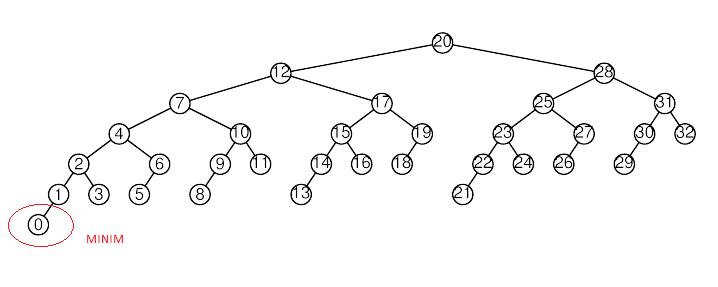
\includegraphics[scale=1]{Min}

\subsection{Performan't'a Find Maximum}
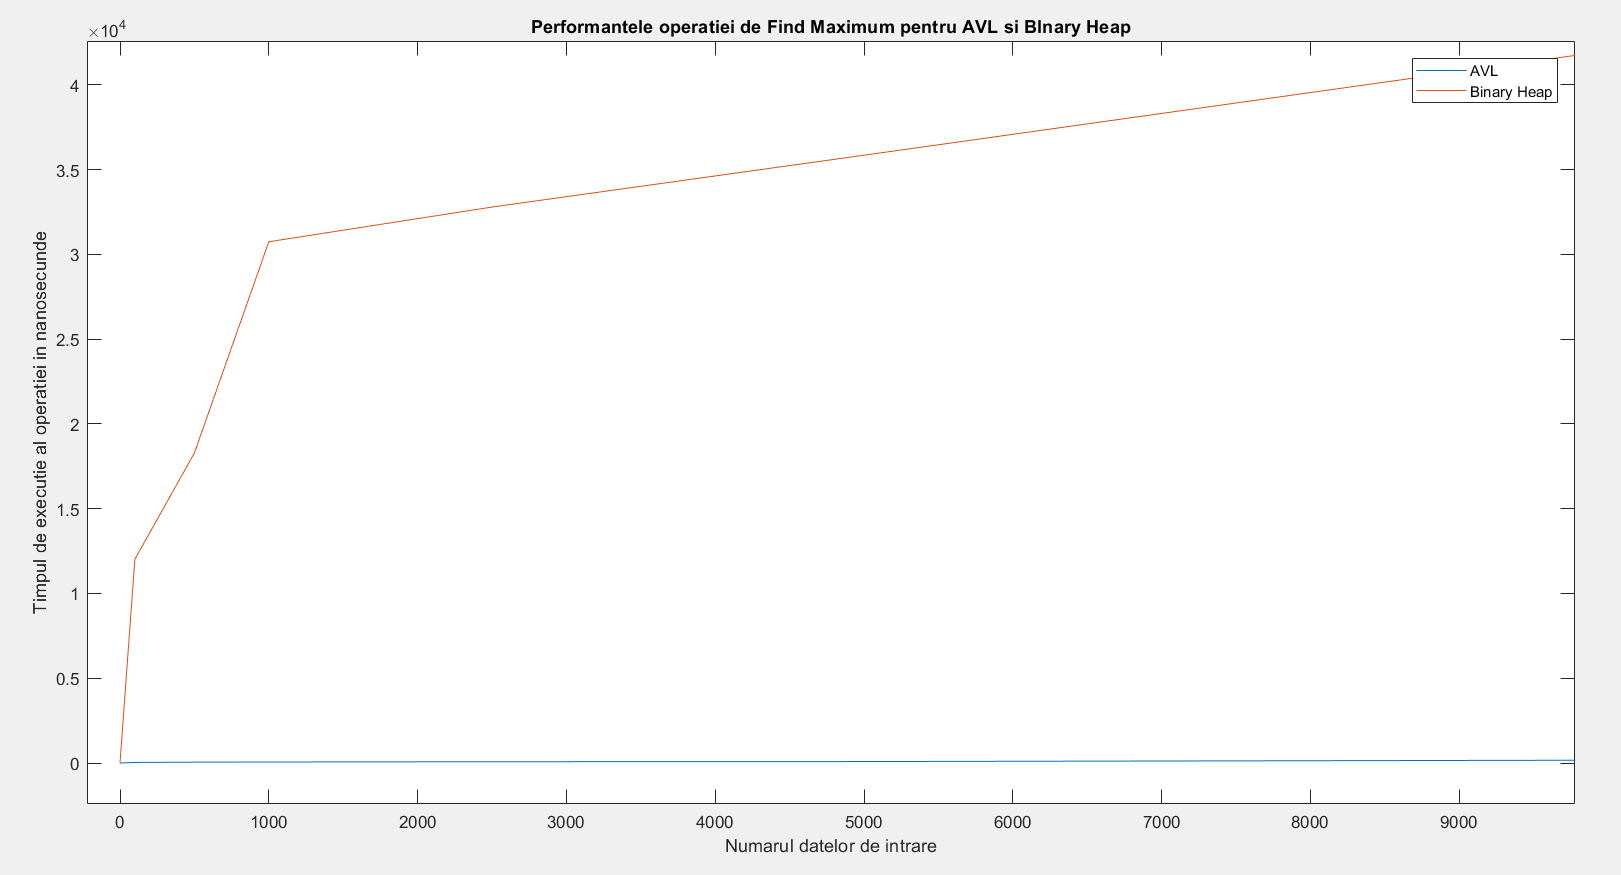
\includegraphics[scale=0.5]{FM}
\\ \par 'In urma test'arii performan'tei pentru opera'tia de c'autare a elementului maxim, am ob'tinut graficul de mai sus, 'in care durata de execu'tie a progrmului este 'in nanosecunde.
\par 'In acest grafic se observ'a timpul foarte mare de care are nevoie un Binary Heap (MinHeap) pentru a g'asi un element din interiorul arborelui. Acesta trebuie s'a caute 'in intreg array-ul pentru a g'asi elementul dorit, pe c\^and, la AVL, acesta va merge pe subarborele drept p\^an'a va g'asi ultimul element frunz'a, care va fi maximul din acel arbore.
\par 'In urm'atoare imagine se poate observa pozi'tia elementului maxim din interiorul unui AVL, precum am explicat anterior.
\\
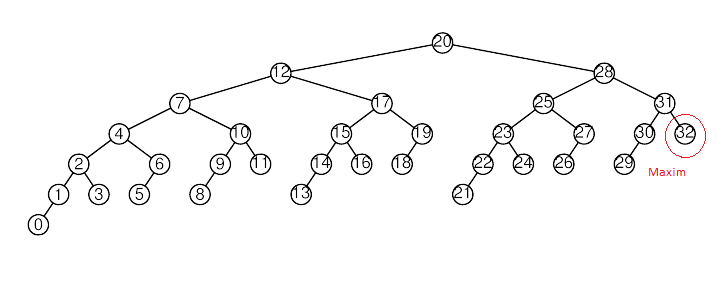
\includegraphics[scale=1]{Maxim}
\subsection{Performan't'a Delete Minimum}
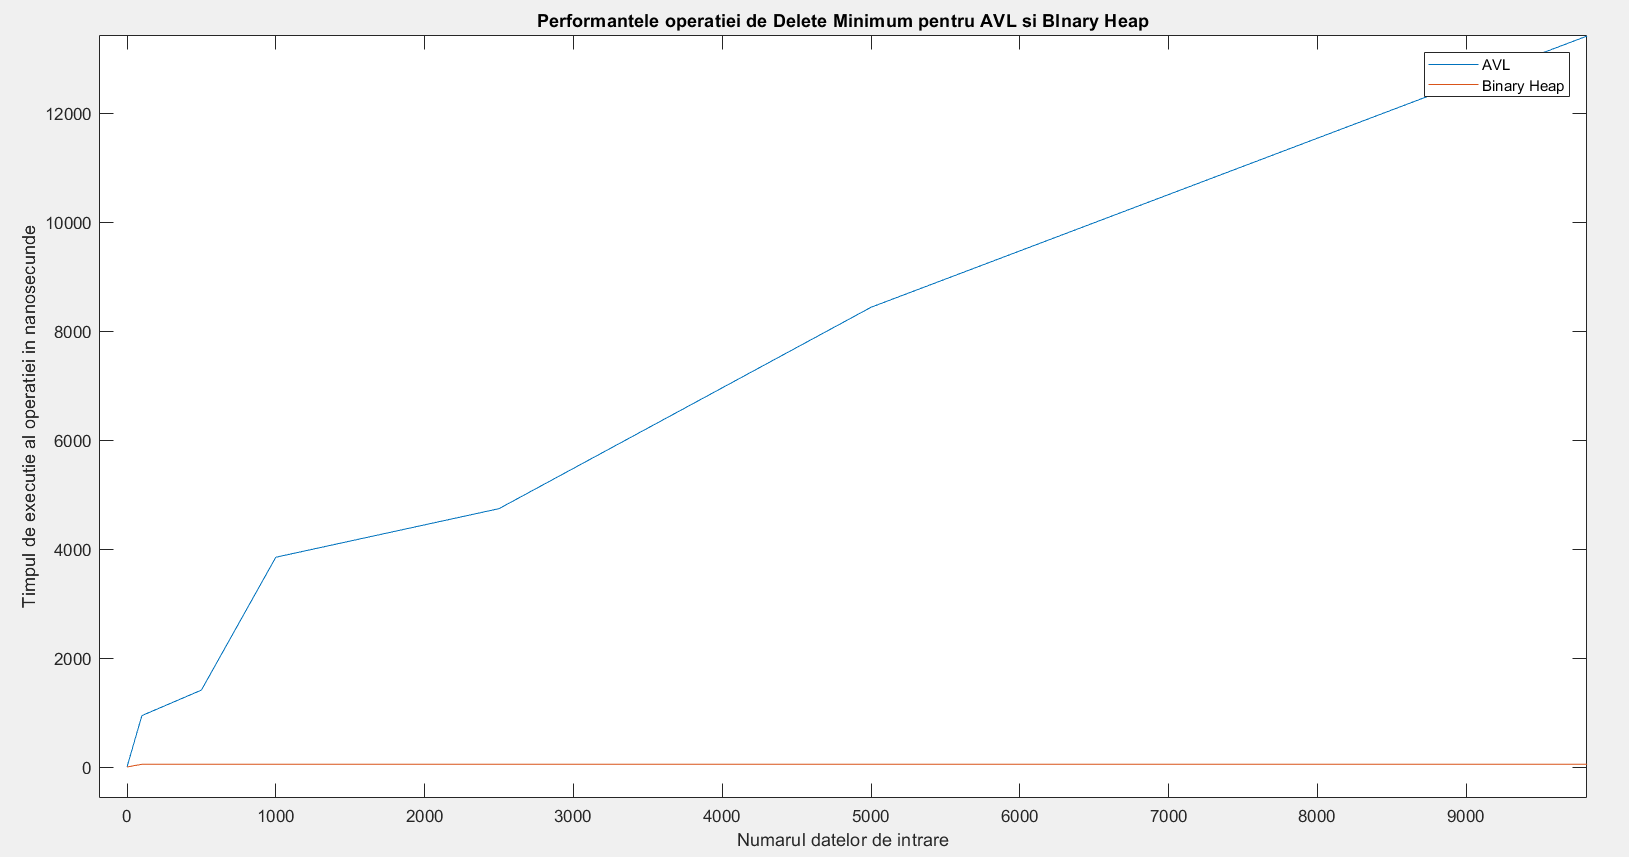
\includegraphics[scale=0.5]{DMin}
\\ \par 'In urma test'arii performan'tei pentru opera'tia de 'stergere a elementului minim, am ob'tinut graficul de mai sus, 'in care durata de execu'tie a progrmului este 'in nanosecunde.
\par Pe acest grafic se observ'a eficien'ta elimin'arii elementului minim dintr-un Binary Heap, aflat pe pozi'tia 0 din array, precum am men'tionat anterior, la Performan'ta Find Minimum (pe cazul implementat MinHeap). Timpul de execu'tie 'in Binary Heap este dat de necesitatea 'inlocuiri root-ului cu succesorul acestuia. 
\par Pentru a elimina elementul minim dintr-un AVL, acesta va parcurge arborele st\^ang p\^an'a se va ajunge la acesta, se va elimina 'si va trebui s'a se realizeze echilibrare, dac'a este nevoie.

\subsection{Performan't'a Delete Maximum}
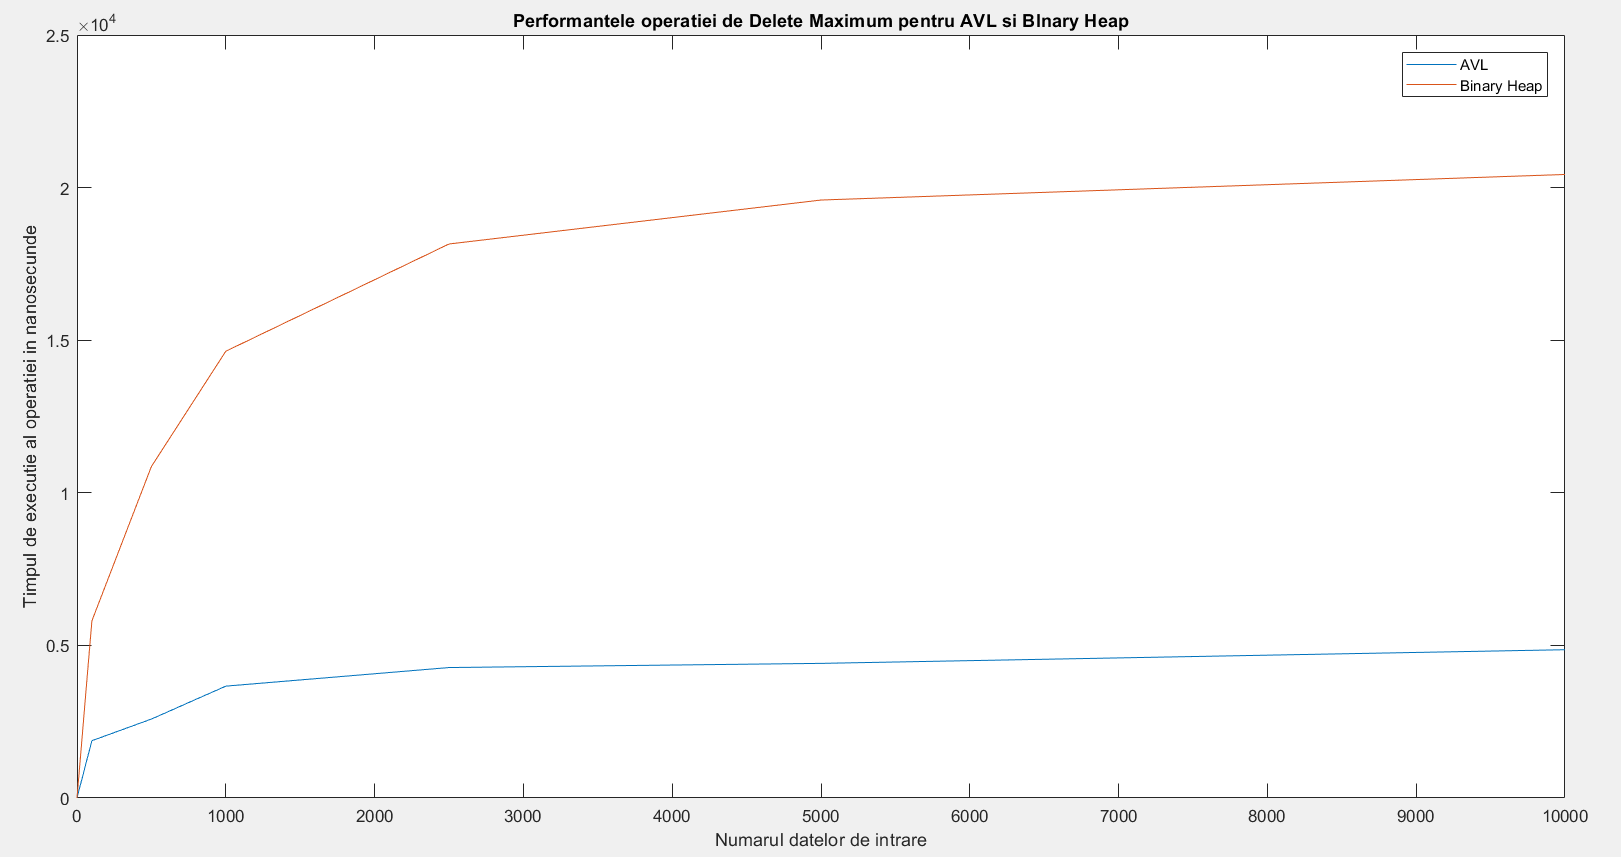
\includegraphics[scale=0.5]{DM}
\\ \par 'In urma test'arii performan'tei pentru opera'tia de 'stergere a elementului maxim, am ob'tinut graficul de mai sus, 'in care durata de execu'tie a progrmului este 'in nanosecunde.
\par 'In acest grafic se observ'a c\^at de mult dureaz'a iterarea pentru un BInary Heap s'a itereze prin 'intreg array-ul pentru a g'asi elementul dorit 'si 'inlocuirea acestuia cu elementul corespunz'ator pentru a p'astra proprietatea arborelui.
\par AVL-ul va parcurge subarborele drept p\^an'a va ajunge la nodul frunz'a 'si va elimina elementul, realiz\^and mai apoi, echilibrarea, daca'a este nevoie.

\newpage
\section{Concluzie}
\par 'In urma analizei prezentate 'in paginile anterioare, putem concluziona c'a nu putem spune despre unul din cei doi algoritmi este superior fa't'a de cel'alalt pe toate planurile.
\par AVL este o structur'a foarte bun'a 'in cazul 'in care nu avem nevoie s'a ada'ug'am de prea multe ori elemente pe parcursul folosirii acesteia 'si cel mai important, dorim s'a facem foarte multe interog'ari, 'in c'autarea elementelor din interiorul structurii. Fiind un arbore binar echilibrat, 'in'al'timea arborelui este logN, iar c'autarea elementelor se face destul de rapid, deoarece cunoa'stem c'a fiul drept al unui nod este reprezentat de o valoare mai mare dec\^at nodul, iar fiul st\^ang al unui nod, este reprezentat de o valoare mai mic'a dec\^at acesta.
\par Binary Heap este o structur'a ce adaug'a elemente destul de rapid. Dac'a la finalul array-ului, unde a fost introdus noul element, se va afla conform propriet'a'tilor Binary Heap-ului, aceast'a inserare este chiar de complexitate $\mathcal{O}(1)$. De asemenea, atuul acestei structuri este dat de accesul 'in $\mathcal{O}(1)$ asupra elementului maxim (MaxHeap) 'si minim (MinHeap). Acest lucru face ca structura s'a fie ideal'a pentru cazuri practice 'in care 'stii c'a este nevoie de interog'ari repete asupra minimului/maximului, precum statistici.





\newpage
\section{Anex'a implement'ari}
\subsection{AVL}
\lstinputlisting[language=Java]{cod/AVL.java}
\subsection{Binary Heap}
\lstinputlisting[language=Java]{cod/BinaryHeap.java}


\newpage
\begin{thebibliography}{2}
\bibitem{AVL}
AVL tree
\\
\href {http://www.geeksforgeeks.org/avl-tree-set-1-insertion/}{http://www.geeksforgeeks.org/avl-tree-set-1-insertion/}  
\\
\bibitem{BIN}
Binary Heap
\\
\href {http://www.sanfoundry.com/java-program-implement-binary-heap/}{http://www.sanfoundry.com/java-program-implement-binary-heap/} 
\\
\bibitem{ran}
Random generator
\\
\href {https://www.random.org/strings/}{https://www.random.org/strings/} 
\\
\end{thebibliography}

\end{document}
